\section{Experiments}
\label{sec:experiments}

% fix algorithm shortcuts, add greedy and brute to the supplement
We apply Two Stage Isometry Pursuit to the standard Iris and Wine datasets, as well as the Ethanol dataset from \citet{Koelle2022-no}.
The latter is an interpretability dataset where a dictionary of precomputed interpretable features are evaluated for their ability to parameterize the data manifold.
Preprocessing details such as tangent space estimation are shared with \citet{Koelle2022-no}.

We use the CVXPY Python package.
We use the SCS interior point solver from CVXPY, which is able to push sparse values arbitrarily close to 0 \cite{cvxpy_sparse_solution}.

\begin{figure}
\centering
\subcaptionbox{Boxplot of $\widehat S_{g}$. \label{fig:boxplot1}}
{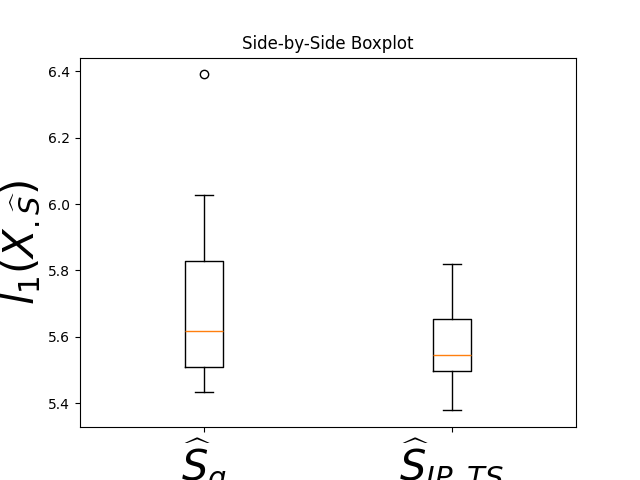
\includegraphics[width=.3\textwidth]{/Users/samsonkoelle/convexlocalisometry/figures/Figure2b.png}}
\subcaptionbox{Boxplot of $\widehat S_{TS}$. \label{fig:boxplot2}}
{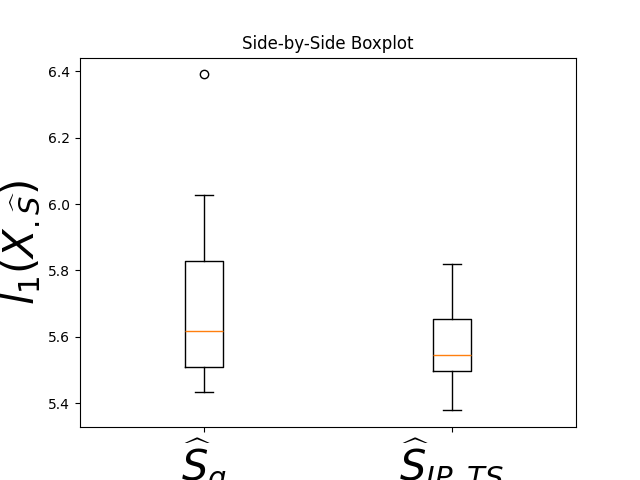
\includegraphics[width=.3\textwidth]{/Users/samsonkoelle/convexlocalisometry/figures/Figure2b.png}}
\subcaptionbox{Boxplot of $\widehat S_{third}$. \label{fig:boxplot3}}
{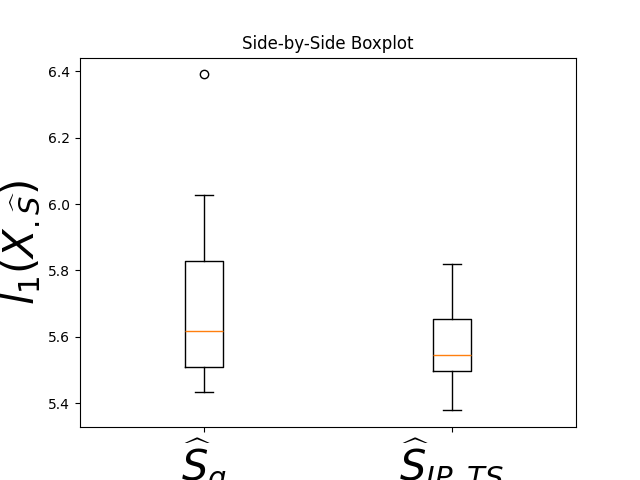
\includegraphics[width=.3\textwidth]{/Users/samsonkoelle/convexlocalisometry/figures/Figure2b.png}}
\caption{Comparison with isometry loss.}
\label{fig:boxplots}
\end{figure}
